\documentclass{document}


\usepackage{url}
\usepackage{rotating}
\usepackage{color}
\usepackage{graphicx}
\graphicspath{ {images/} }


\begin{document}

\title[Is Ensembling Always Preferable for Medical Data?]{Does Ensembling Classifiers Always Confer a Quantifiable Advantage over Selecting a Single Best Classifier for Medical Diagnosis or Prognosis?}

\section{Titlepage}



\abstract{\textbf{Motivation:} Rapid expansion of the amount of medical data available to the healthcare industry is driving demand for more accurate, precise and reliable tools for exploiting these data. Real-world experience suggests that combining the predictions of individual machine-learning classifiers may allow us to meet all three criteria at a low cost, potentially saving scarce funds and patients' lives. We therefore attempt to go beyond the existing literature on individual machine learning algorithms to discover the effectiveness of combining their predictions, and to explore the potential benefits of such 'ensemble methods' to personalised diagnostic and prognostic medicine.\\
\\
\textbf{Results:} 
Consideration of a range of classifiers is an important aspect in getting the best predictive performance for a given data set.  For each of the 10 biomedical data sets considered in this paper, a range of classifier ensemble methods performed competitively with respect to individual classifiers. Furthermore, it was possible to reliably automate the ensemble methods, making them straightforward to apply to new data sets.  It was noteworthy that unsupervised methods such as averaging of prediction probabilities generally performed well despite their simplicity.  Strikingly, we found that simply selecting the best-performing individual model was actually a very strong strategy, outperforming most of the model 'blending' approaches leading to best or near-best predictive performance on all 10 data sets.
\\
We conclude that while it is clearly important to consider a range of classifiers for a given data set, simple strategies such as selecting the best-performing bas classifier should not be discounted.  We also speculate that  the widely observed predictive performance improvements seen in e.g. data science competitions may be more the result of averaging over different set of features and feature representations, rather than over different types of model.  We then conclude that there may be significant merit in the development of formal methods for selecting between a wide range of different classifiers.
\\
\textbf{Availability:} R implementations of our own base and ensemble classifiers are available at \url{https://github.com/christensen5/Classifiers-for-Medical-Machine-Learning.git}\\
A Python implementation of Edwin Simpson's IBCC classifier is available at \url{https://github.com/CitizenScienceInAstronomyWorkshop/pyIBCC}}

\maketitle

\section{Keywords}
\textcolor{red}{KEYWORDS HERE}


\section{Background}
As medicine continues to evolve into a data-rich discipline, there is an increasing need for machine learning methods which can take full advantage of the rapidly-growing data volumes that doctors are amassing on their patients and the illnesses which afflict them. In non-medical applications of machine learning, such as the well-known Netflix competition\textcolor{red}{\cite{netflixprize}}, it is often the case that incremental gains in performance are not worth the extra computational cost, but the nascent  field of personalised medicine is particularly well-placed to benefit from even  relatively modest improvements in  predictive performance, since early  and precise identification of a disease can save both treatment costs and patients' lives. 

Ensemble methods have been seen to offer noticeable performance gains over individual classification algorithms in a multitude of real-world scenarios 
\textcolor{red}{e.g. \url{www.netflixprize.com}, \url{https://www.kaggle.com/competitions}}, 
however it is unclear precisely from what aspect of the ensembling this improved performance stems.  It is therefore important to determine more precisely if and when these gains can be exploited by the medical community.

There exists already a significant amount of literature studying the variety and effectiveness of individual machine learning classifiers (see \cite{classifiercomparison} for one exhaustive example). In practise, real-world results suggest that it is usually possible to obtain a statistically significant boost in predictive ability by combining the predictions from a number of different learners. Such combination methods (which we shall refer to as "ensemble methods" or "ensemble classifiers") exist in many forms, from simple averaging of predictions or majority voting, to more complex so-called "meta-learning" approaches. Our task is to obtain data on the performance of a variety of such ensemble classifiers on a collection of medical datasets, in order to evaluate whether or not ensembling does in general offer a genuine performance increase.


\section{Methods}

 We aim to assess the effectiveness of different combination strategies compared to each other and to the individual classification algorithms whose predictions they employ.  We focus on datasets of a medical nature in order to obtain results specifically relevant to the field of diagnostic and prognostic medical machine learning.

We have assembled a collection\footnote{These datasets also form part of the collection of datasets in Fernandez-Delgado's paper \cite{classifiercomparison} comparing base classifiers.} of datasets from the UCI machine learning repository, selected for meeting the following conditions:

\begin{itemize}
\item Data of a medical nature
\item Binary  outcome variable
\item At least 250 instances without missing data
\end{itemize}

\noindent
We use a collection of 11 base classifiers (drawn from a variety of existing R packages) and 7 ensemble classifiers (both existing and of our own implementation) to train and obtain predictions. The predictions of each ensemble classifier on each dataset are evaluated by the AUC metric to determine their effectiveness compared to each other and to the best performing base classifier on that dataset.

All of the classifiers with the exception of the Independent Bayesian Classifier Combination (IBCC) ensemble are run in R. IBCC is run in Python using the implementation given in \cite{Simpson13}. In order to avoid bias, predictions are created independently before being passed to any ensemble classifier, and all were given the same set of predictions for each data set, whether via R or via Python.


\subsection{Datasets}

We  used the following data sets in our comparison, all taken from the UCI machine learning repository\cite{UCIrep}.

\begin{enumerate}
    \item \textbf{Breast Cancer Wisconsin (Original)} (1991): classification of tumours into 'benign' or 'malignant'. Courtesy of Dr. William H Wolberg, Universiy of Wisconsin Hospitals, Madison.
    \item \textbf{Breast Cancer Wisconsin (Diagnostic)} (1994): classification of tumours into 'benign' or 'malignant'. Courtesy of Dr. William H. Wolberg, University of Wisconsin, Clinical Sciences Center, Madison.
    \item \textbf{Haberman's Survival Dataset} (1999): classification of patients undergoing breast cancer surgery into 'deceased within 5 years' or 'survived at least 5 years'. Courtesy of University of Chicago's Billings Hospital \& Tjen-Sien Lim, Department of Statistics, University of Wisconsin, Madison.
    \item \textbf{Heart Disease Dataset (Hungarian)} (1988): classification of patients into 'presence' or 'absence' of heart disease. Courtesy of Andras Janosi, M.D., Hungarian Institute of Cardiology, Budapest \& David W. Aha, Institute of Information and Computer Science, UCI.
    \item \textbf{Indian Liver Patient Database} (2012): classification of patients into 'liver patient' or 'non liver patient'. Courtesy of B. V. Ramana \& Prof N. B. Venkateswarlu, Aditya Institute of Technology and Management \& Prof M. S. Prasad Babu, Andhra University College of Engineering.
    \item \textbf{Mammographic Mass Dataset} (2007): classification of mammographic masses into 'benign' or 'malignant'. Courtesy of Matthias Elter, Fraunhofer Institute for Integrated Circuits, Erlangen, Germany \& Dr Rudiger Schulz-Wendtland, Institute of Radiology, University Erlangen-Nuremberg, Germany.
    \item \textbf{Single Proton Emission Computed Tomography (SPECT) Heart-imaging Dataset} (2001): classification of SPECT heart images into 'normal' or 'abnormal'. Courtesy of Krzysztof J. Cios \& Lukasz A. Kurgan, University of Colorado, Denver \& Lucy S. Goodenday, Medical College of Ohio, Ohio.
    \item \textbf{SPECTF Heart-imaging Dataset} (2001): classification of SPECTF heart images into 'normal' or 'abnormal'. Courtesy of Krzysztof J. Cios \& Lukasz A. Kurgan, University of Colorado, Denver \& Lucy S. Goodenday, Medical College of Ohio, Ohio.
    \item \textbf{Statlog (Heart) Dataset} : classification of patients into 'presence' or 'absence' of heart disease. Source anonymised by UCI.
    \item \textbf{Vertebral Column Dataset} (2011): classification of orthopaedic patients into 'normal' or 'abnormal'. Courtesy of Guilherme de Alencar Barreto \& Ajalmar da Rocha Neto, Department of Teleinformatics Engineering, Federal University of Ceará, Fortaleza, Brazil \& Dr. Henrique da Mota Filho, Hospital Monte Klinikum, Fortaleza, Brazil.
\end{enumerate}

The following table provides further details of each of the above datasets, each of which is henceforth referred to by a shortened label or acronym, in the interest of compactness.

\begin{table}[b]
\centering
\begin{tabular*}{8cm} {@{}c @{\extracolsep{\fill}} ccc@{}}
\hline
datasets        & \#instances  &\#variables & Majority\%\\
\hline
bc-wisc-original&       683    &   9        &   52.2\\ 
bc-wisc-diag    &       569    &   30       &   62.7\\ 
haberman-survival&      306    &   3        &   73.5\\
heart-hungary   &       261    &   10       &   62.5\\
ilpd-indian-liver&      579    &   10       &   71.5\\
mammographic    &       830    &   4        &   51.4\\
spect           &       267    &   22       &   79.4\\
spectF          &       267    &   44       &   79.4\\
st-heart        &       270    &   13       &   55.6\\
vertebral-col   &       310    &   6        &   67.7\\
\hline
\end{tabular*}
\caption{Our collection of 10 datasets from the UCI repository. Columns represent the number of instances, number of variables and the percentage of the majority class for each of the datasets after missing data is removed. Further detail on each dataset can be found in the list following the table.}
\label{table:datasets}
\end{table}

\subsection{Data Conversion \& Processing}

Missing data have been removed from the datasets, either by removing only the single instance with the missing data point or by removing an entire variable in the few cases where data for a specific variable is missing for all but a very small number of instances.

In the cases where non-numeric values are given (e.g. M/F to represent gender) a simple numeric conversion is applied: if a variable $x$ can attain (discrete) non-numeric values $\{a_{1}, a_{2}, ..., a_{n}\}$ then the value $a_{i}$ is converted to the number $i \in \{1,...,n\}$.

Before being passed to the k-NN base classifier, each variable is processed to have zero mean and standard deviation one. Since k-NN is a distance-based classifier, variables will be weighted according to the size of the range in their numerical values, rather than according to any genuine underlying medical importance. We therefore apply this pre-processing to 'smooth out' this weighting more uniformly. We apply the same normalisation before passing data to the Neural Network base classifier, following best practise for this kind of classifier. We do not use further pre-processing, data transformation or feature selection.


\subsection{Base Classifiers}

We use the following Base Classifiers, implemented in R, to obtain predictions on which to train and test ensemble methods.

\begin{enumerate}

    \item \textbf{Sparse Logicstic Regression}, using \textit{cv.glmnet} in the \textit{glmnet} package. We run with the flags \textit{maxit=1e5, alpha=1, family="binomial"}.
    \item \textbf{Random Forest}, using \textit{randomForest} in the \textit{randomForest} package. We run with the flags \textit{importance=TRUE, ntree=1500}.
    \item \textbf{Generalised Boosting Model}, using \textit{gbm} in the \textit{gbm} package. Flags \textit{distribution="bernoulli", ntrees=3000, interaction.depth=4, cv.folds=3, n.cores=2, n.minobsinnode < 10}.
    \item \textbf{Gaussian Process}, using \textit{gausspr} in the \textit{kernlab} package. We use set.seed to obtain consistent results in the interests of obtaining results that reflect the classification ability of the ensembling methods, not of the underlying base classifiers. Flags \textit{kernel="rbfdot"}.
    \item \textbf{Support Vector Machine}, using \textit{ksvm} in the \textit{kernlab} package. Flags \textit{kernel="rbfdot", prob.model=TRUE, kpar=list(sigma=0.05), C=5, cross=3}.
    \item \textbf{Neural Network}, using \textit{neuralnet} in the \textit{neuralnet} package. Flags \textit{hidden=1, threshold=0.01, linear.output=FALSE}.
    \item \textbf{Decision Tree}, using \textit{C5.0} in the \textit{C50} package. Flags \textit{trials=1, rules=FALSE}.
    \item \textbf{Rule-Based Method}, using \textit{C5.0} in the \textit{C50} package. Flags \textit{trials=1, rules=TRUE}.
    \item \textbf{k-Nearest Neighbour}, using \textit{knn3} in the \textit{caret} package. Flags \textit{k=40}.
    \item \textbf{Naive Bayes}, using \textit{NaiveBayes} in the \textit{klaR} package.
    \item \textbf{Linear Discriminant Analysis}, using \textit{lda} in the  \textit{MASS} package. 
\end{enumerate}


\subsection{Ensembling Process}
\label{ensemblingprocess}

Each dataset is partitioned randomly into three subsets:
\begin{enumerate}
\item Btrain (base classifier training set, 50\% of data instances)
\item Mtrain (ensemble classifier training set, 25\% of data instances)
\item Mtest (ensemble classifier testing set, 25\% of data instances)
\end{enumerate}

\noindent
The ensemble predictions are obtained through the following procedures:

\vspace{1cm}
\noindent
\textbf{Ensemblers with no meta-learning stage:}
First, the base classifiers are trained on the combined set Btrain $\cup$ Mtrain, and predictions for Mtest are obtained. These predictions are passed to the ensemble classifier, to combine into a final set of predictions.

\noindent
\textbf{Ensemblers with a meta-learning stage:}
First, the base classifiers are trained on the set Btrain, and separate predictions for Mtrain and Mtest are computed. The predictions for Mtrain are passed to the ensemble classifier to train the meta-learner, which then is given the predictions for Mtest in order to ensemble them into a final set of predictions.


\subsection{Ensemble Classifiers}

To ensemble the base classifier predictions, we use the following Ensemble Classifiers, implemented in R (with the exception of IBCC, for which the Python implementation in \cite{Simpson13} is used).

\begin{enumerate}
    \item \textbf{Average}, simple average of the probabilistic base classifier predictions for each instance. No meta-learning stage is needed by this method.
    \item \textbf{Weighted Average}, as with Average, but with a meta-learning stage in which each contributing base classifier has its prediction weighted according to its AUC score when classifying Mtrain.
    \item \textbf{Majority Vote}, converts probabilistic base classifier predictions to "votes" (binary 0/1 predictions) by rounding. Then combines the votes for each instance by summing them all and dividing by the number of instances to obtain a prediction between 0 and 1. No meta-learning stage.
    \item \textbf{Rank Average}, ranks the predictions for each base classifier separately, then normalises these to obtain uniformly spaced values between 0 and 1, before computing a simple average of the ranks for each instance. No meta-learning stage.
    \item \textbf{Stacking w/ Logistic Regression} uses glm, a logistic regression algorithm from the \textit{stats} package, as a meta-classifier, learning to ensemble the base classifier predictions for Mtrain, and returning ensembled predictions for Mtest. Flags \textit{family="binomial"}.
    \item \textbf{Stacking w/ Sparse Logistic Regression} uses glmnet from the \textit{glmnet} package, as a meta-classifier, learning to ensemble the base classifier predictions for Mtrain, and returning ensembled predictions for Mtest. Flags \textit{family="binomial", maxit=1e5, alpha=1}
    \item \textbf{Stacking w/ Random Forest} uses randomForest from the \textit{randomForest} package, as a meta-classifier, learning to ensemble the base classifier predictions for Mtrain, and returning ensembled predictions for Mtest. Flags \textit{importance=TRUE, ntree=500}
    \item \textbf{IBCC} (supervised mode), "Bayesian classifier combination, using the computationally efficient framework of variational Bayesian inference."\cite{Simpson13}. In supervised mode, IBCC acts as a meta-classifier, learning to ensemble the base classifier predictions.
    \item \textbf{IBCC} (unsupervised mode). In unsupervised mode, IBCC performs unsupervised learning on the predictions obtained by training the base classifiers on the combined set Btrain $\cup$ Mtrain, thereby learning to ensemble base classifier predictions.
\end{enumerate}


\subsection{Comparison Metric}

The performance of the classifiers is evaluated using the AUC metric, implemented in R using the roc function from the \texttt{pROC} package. For each classifier we use this function to obtain the AUC and a 95\% confidence interval. Tables including all of these data are included at the end of the document, in Tables \ref{fig:04} \& \ref{fig:05}.



\section{Results \& Discussion}
\label{results&discussion}

In our experimental analysis we evaluate 9 ensemble methods, combining the predictions of 11 base classifiers over 10 datasets. We find that one of our base classifiers (NaiveBayes) strictly requires non-zero variances for all variables, and therefore will return errors when analysing the spect (but not spectF) dataset. We therefore omit the NaiveBayes base classifier when obtaining predictions for the spect dataset.

\noindent
Figure \ref{fig:01} displays the  AUC scores of each base classifier on each dataset. We include this for two principal reasons; firstly to demonstrate that the base classifiers are reasonably effective on their own, and therefore our ensembles are not "polluted" by including routinely impotent base predictions, and secondly to demonstrate that there is nonetheless a significant range in performance across datasets and classification algorithms. As the famous "No Free Lunch" Theorems would lead us to expect, we do not observe that any particular base classifier performs best on every dataset (or even a significant majority of them), but there are naturally some which tend to perform well by comparison to the rest.

\noindent
Figure \ref{fig:02} displays the  AUC scores of each ensemble classifier on each dataset. It was to be expected (once again in accordance with the "No Free Lunch" principle) that no individual ensemble method would prove consistently superior to the others. Our aim, therefore, is rather to determine whether or not it is usually possible to obtain an improvement in accuracy over the base classifiers by implementing \emph{some kind} of ensembling (i.e. is there usually at least one ensemble classifier which outperforms the best base classifier?). Conventional wisdom and the results from many real-world applications of machine learning (in particular competitions such as the Netflix Prize\cite{netflixprize} and Kaggle competitions\cite{kagglecompetitions}) suggest that a noticeable improvement is usually possible using even relatively unsophisticated ensembling techniques.

We are therefore surprised to note that our results suggest that the best base classifier surpasses the accuracy of every ensemble classifier on 5 of our 10 datasets, and equals the accuracy of the best ensemble classifier on a further 2 datasets. Stacking with some form of logistic regression as the meta-learner is the only ensembling approach that manages to outperform the best base classifier on any of the datasets. This suggests that perhaps ensembling for model uncertainty as we have done here is less important than selecting the best base classifier for a given task (as stacking is broadly attempting to do).

\noindent
We observe also a few general trends:

\begin{enumerate}
\item Average and Stack SLR are the stand-out best performers amongst the ensemble methods, with Rank Average also showing strong results.
\item Average performs in the top 3 ensemble classifiers on 8 out of 10 datasets (although it never outperforms the best base classifier) and does not perform catastrophically on any of the datasets (unlike some of the more sophisticated ensemble methods), displaying a respectable level of consistency. These observations are also true to a slightly lesser extent for the similar Rank Average ensemble.
\item Stacking with sparse logistic regression (as in Stack SLR) significantly outperforms stacking with logistic regression (as in Stack LR) on every dataset except st-heart. It seems that there is some aspect of these kinds of dataset which Stack SLR is generally better able to capture than Stack LR.
\item Unsupervised IBCC significantly outperforms Supervised IBCC on 7 of our 10 datasets, and on the 2 datasets where Supervised IBCC wins, it does so by a much smaller margin.
\item Along the same lines as the previous point, the ensemble classifiers which forego a meta-learning stage in favour of a larger base classifier training set generally exhibit a respectable performance both in terms of AUC score and consistency.
\end{enumerate}

\noindent
The contrasting nature of the ensemble methods which include a meta-learing stage and those which do not, leads to a difference in the way that data is fed to each. As explained in Section \ref{ensemblingprocess}, for an ensemble classifier which does not require the training of a meta-learning on the Mtrain subset, we opt instead to include Mtrain along with Btrain in the training data for the base classifiers, for two reasons. Firstly, to withold the subset Mtrain completely from these ensemble classifiers would be to impose on them a data deficit in comparison to the meta-learning ensemblers, resulting in an unfair comparison. Secondly, any real-world implementation of these ensemble classifiers would surely aim to make full use of the available data, rather than arbitrarily withholding a 25\% subset, so for the purposes of obtaining results that are applicable to real-world best practise, ours is the more reasonable approach. Figure \ref{fig:03} supports these assertions, demonstrating that a larger base classifier training set almost universally results in significantly greater prediction accuracy.


\vspace{-5mm}
\section{Conclusion}

The most immediate conclusion to be drawn from our results is that ensembling for model uncertainty is not always more effective than simply selecting the best base classifier. Indeed, the only ensemble methods to outperform the best base classifier were Stack SLR and Stack LR, both of which work broadly by attempting to 'learn' which are the best base classifiers and then weighting the their predictions the most heavily.

How might this be reconciled with the fact that real-world applications often do show a performance boost from ensembling? We note that many such real-world applications (e.g. Kaggle competition winners and the top performers in the Netflix Prize) include varying degrees of feature learning and ensembling over feature sets, rather than our approach of ensembling over only a set of base classifiers, each applied to exactly the same feature set. This suggests that the observed success of ensembling in these cases may have more to do with these alternative approaches to ensembling - a hypothesis which we believe merits future investigation.

\vspace{0.2cm}
\noindent
Our results suggest also that it is important to consider the 'cost' of some ensemble methods in terms of training data. We see with regards to IBCC that the advantages conferred by meta-learning from labelled training examples in Supervised IBCC appear to be outweighed by the larger volume of training data given to the base classifiers in Unsupervised IBCC. More generally, the relative performance of the meta-learning and non-meta-learning ensemble methods supports the idea that the performance gain from ensembling with a meta-learner may not outweigh the cost of a reduced training set, particularly if the entire dataset is small to begin with, as may often be the case in medical applications. It is therefore clearly important to carefully consider the nature of a dataset, and not just which classifiers to use, when attempting to obtain good predictions.

\vspace{0.2cm}
\noindent
Finally, we mention the respectable performance of the very basic Average and Rank Average ensemble methods, relative to more complex approaches such as stacking, which perform extremely poorly on a small number of the datasets. With regards to medical applications in diagnosis, for example, it is clear to see why one would prefer a consistently good classifier over an occasionally excellent classifier whose consistency varies greatly, even if the latter is sometimes the best performing classifier of all. Furthermore, as the volume of medical data available to doctors increases, it will become increasingly important to consider the computational cost of machine learning methods, in which simpler methods such as Average and Rank Average are clear winners over Stacking and IBCC.

\vspace{-5mm}

\section{List of Abbreviations}
\textcolor{red}{LIST OF ABBREVIATIONS HERE}

\section{Declarations}
	
	\subsection{Ethics}
	\subsection{Consent for publication}
	\subsection{Availability}
	\subsection{Competing Interests}
	\subsection{Funding}
	This work has been supported by University of Warwick's Undergraduate Research Support Scheme (URSS), and by the Systems Biology Centre at the University of Warwick.
	\subsection{Authors' Contributions}
	\subsection{Acknowledgements}
	We thank Edwin Simpson, for providing a complete Python implementation of his IBCC classifier and for useful discussion during the course of our investigation.



%\bibliographystyle{natbib}
%\bibliographystyle{achemnat}
%\bibliographystyle{plainnat}
%\bibliographystyle{abbrv}
%\bibliographystyle{bioinformatics}
%
%\bibliographystyle{plain}
%
%\bibliography{Document}


\clearpage

\begin{figure}[p]
\centering
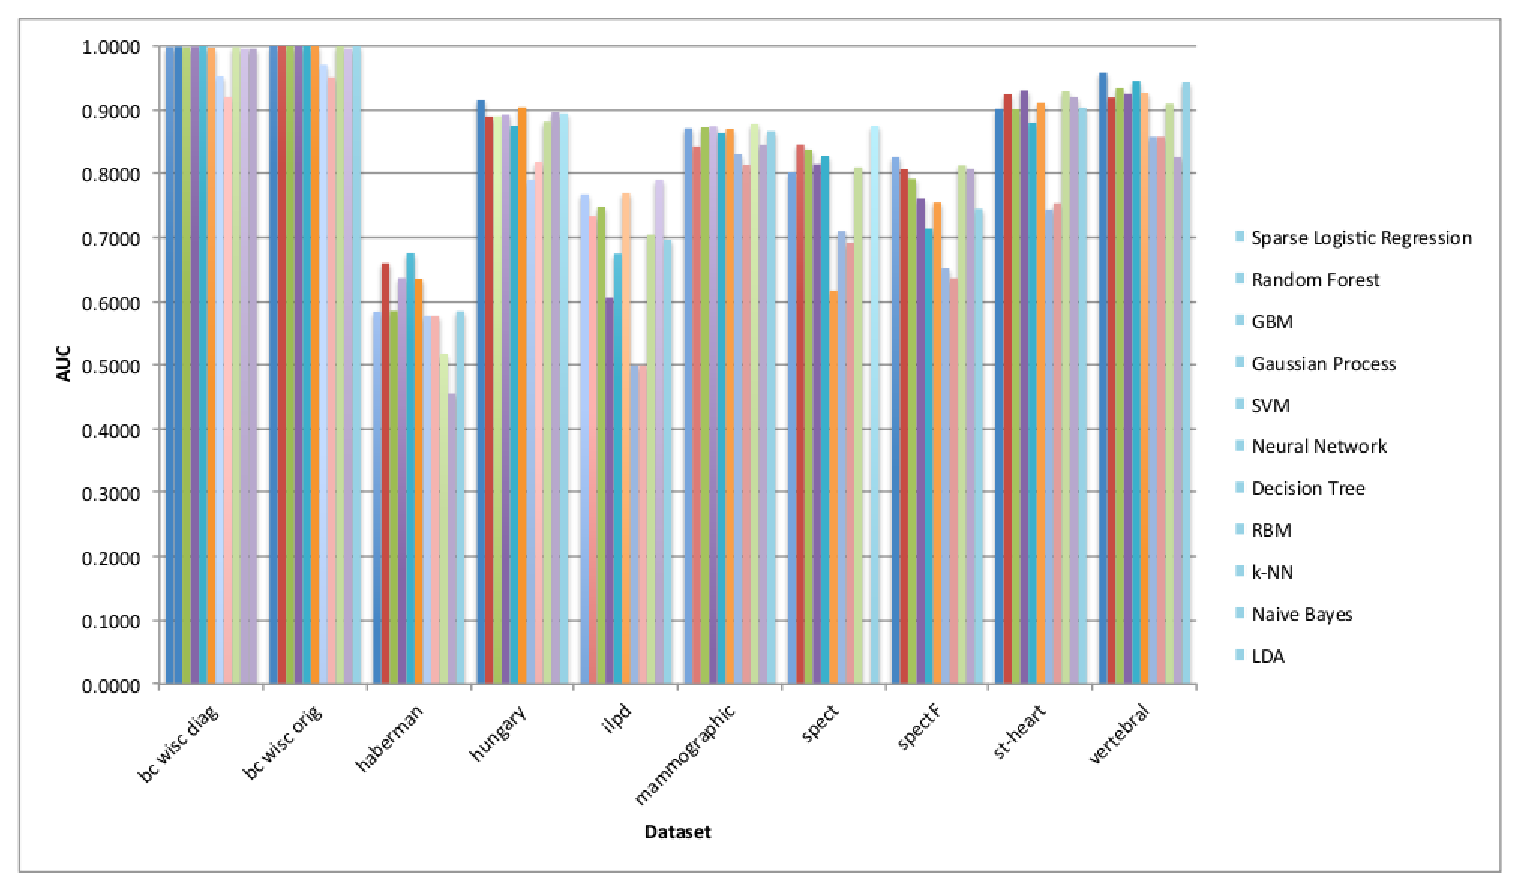
\includegraphics[angle=0, width=175mm]{basegraph.eps}
\caption{Base Classifier Accuracy on a Variety of Datasets}
\label{fig:01}
\end{figure}


\begin{figure}[p]
\centering
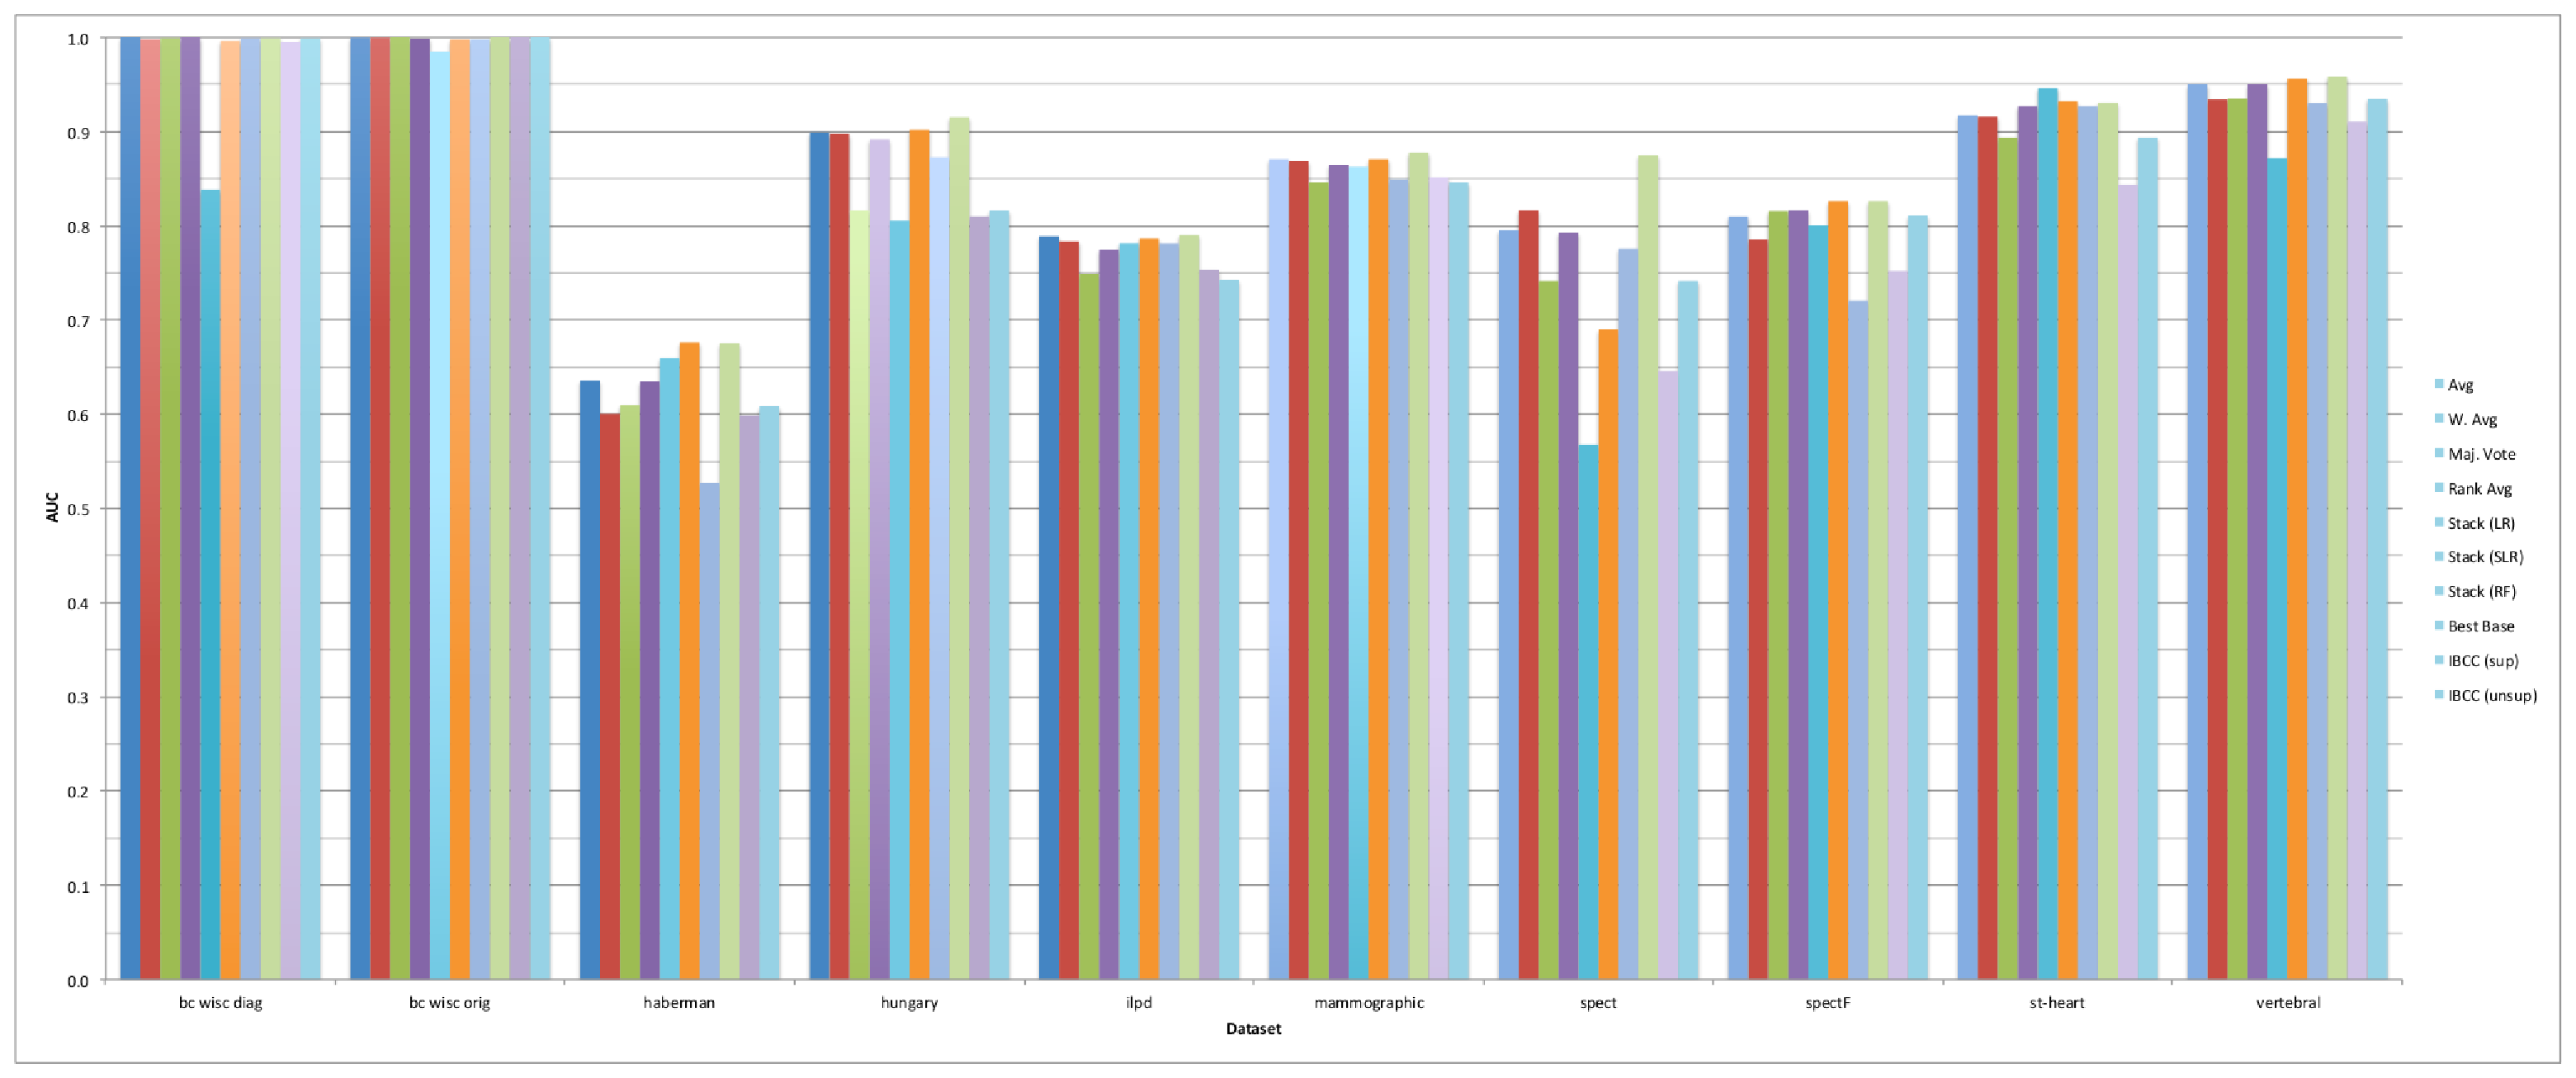
\includegraphics[angle=0, width=175mm]{ensemblegraph.eps}
\caption{Ensemble Classifier Accuracy on a Variety of Datasets}
\label{fig:02}
\end{figure}

\clearpage
\begin{figure}[p]
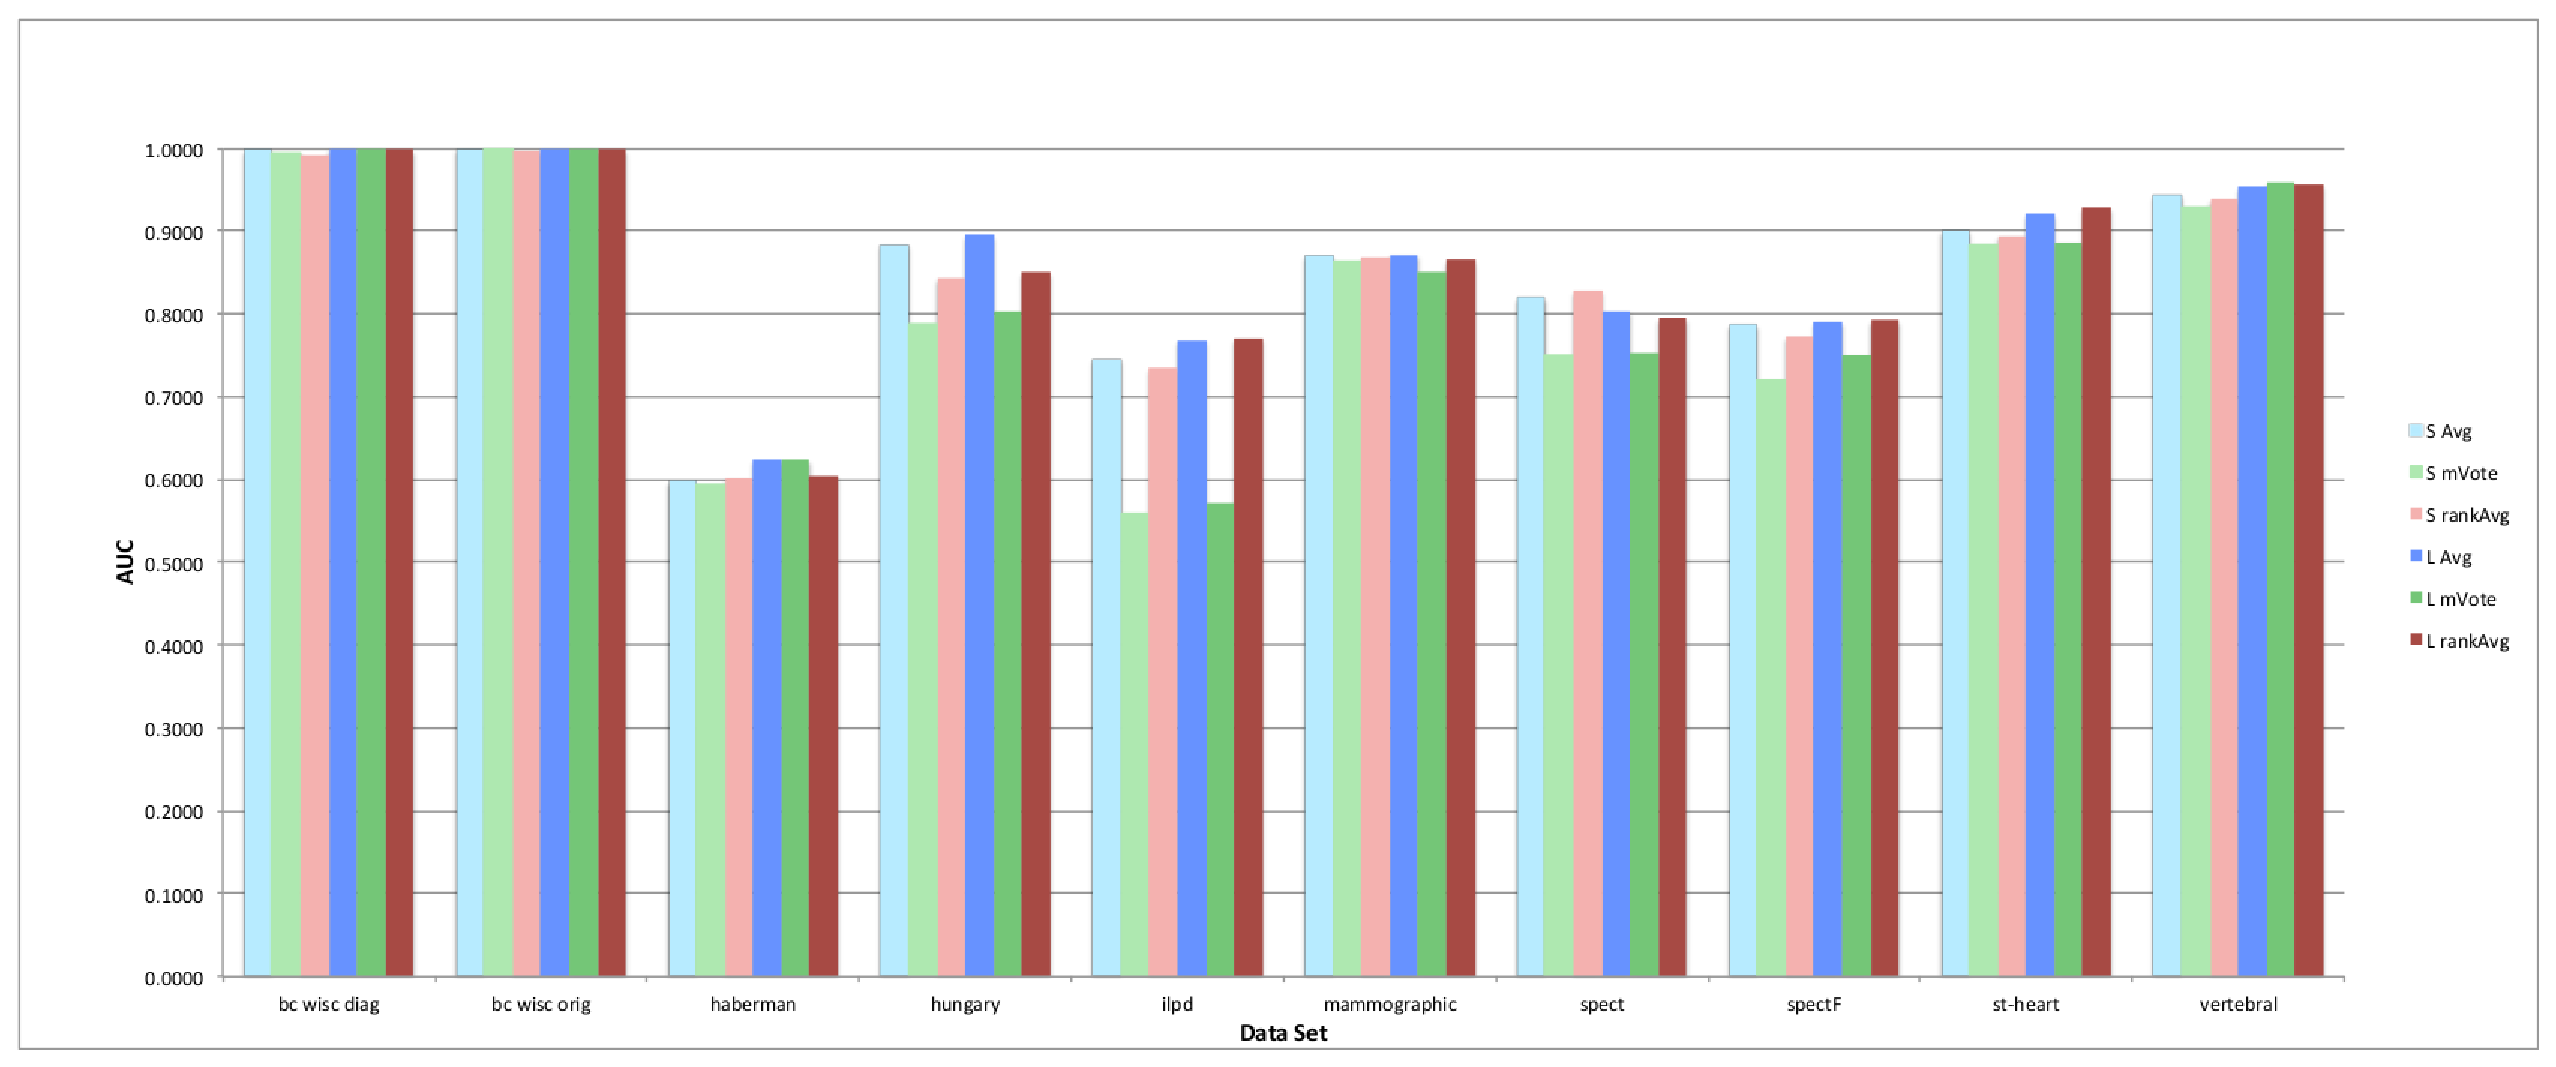
\includegraphics[angle=0, width=175mm]{smallvlargegraph.eps}
\caption{Non-Meta-Learning Ensemble Accuracy on Small (pale colours) vs Large (dark colours) training sets}
\label{fig:03}
\end{figure}




\begin{table}[t]
\centering
\begin{tabular*}{16.5cm}{@{\extracolsep{\fill} } |c||c|c|c|c|c|c|c|c|c|c|}
    \hline
    & \textbf{bc wisc diag} & \textbf{bc wisc orig} & \textbf{haberman} & \textbf{hungary} & \textbf{ilpd} & \textbf{mammographic} & \textbf{spect} & \textbf{spectF} & \textbf{st-heart} & \textbf{vertebral}\\ \hline
    \textbf{glmnet} & 0.9987 & 1.0000 & 0.5839 & 0.9154 & 0.7678 & 0.8713 & 0.8019 & 0.8263 & 0.9018 & 0.9586\\ \hline
    \textbf{rf} & 0.9989 & 1.0000 & 0.6599 & 0.8896 & 0.7338 & 0.8427 & 0.8458 & 0.8068 & 0.9246 & 0.9194\\ \hline
    \textbf{gbm} & 0.9981 & 1.0000 & 0.5851 & 0.8900 & 0.7482 & 0.8726 & 0.8377 & 0.7922 & 0.9009 & 0.9342\\ \hline
    \textbf{gp} & 0.9989 & 1.0000 & 0.6368 & 0.8929 & 0.6062 & 0.8745 & 0.8149 & 0.7614 & 0.9307 & 0.9253\\ \hline
    \textbf{nnet} & 0.9971 & 1.0000 & 0.6351 & 0.9041 & 0.7698 & 0.8703 & 0.6169 & 0.7549 & 0.9114 & 0.9268\\ \hline
    \textbf{dt} & 0.9524 & 0.9708 & 0.5773 & 0.7904 & 0.5000 & 0.8303 & 0.7102 & 0.6518 & 0.7439 & 0.8580\\ \hline
    \textbf{rbm} & 0.9202 & 0.9512 & 0.5773 & 0.8186 & 0.5000 & 0.8139 & 0.6916 & 0.6364 & 0.7539 & 0.8580\\ \hline
    \textbf{knn} & 0.9987 & 1.0000 & 0.5178 & 0.8816 & 0.7047 & 0.8779 & 0.8101 & 0.8133 & 0.9289 & 0.9098\\ \hline
    \textbf{nb} & 0.9958 & 0.9960 & 0.4558 & 0.8966 & 0.7905 & 0.8452 & * & 0.8076 & 0.9202 & 0.8262\\ \hline
    \textbf{lda} & 0.9960 & 1.0000 & 0.5847 & 0.8947 & 0.6970 & 0.8669 & 0.8750 & 0.7451 & 0.9035 & 0.9430\\ \hline
\end{tabular*}
\caption{AUC scores for base classifiers on each dataset. \newline * see Section \ref{results&discussion}.}
\label{fig:04}
\end{table}


\clearpage
\begin{table*}[b]
\small
\begin{tabular}
    {|c|c||c|c|c|c|c|c|c|c|c|c|c|}
    \hline
    && \textbf{Avg} & \textbf{wAvg} & \textbf{mVote} & \textbf{rankAvg} & \textbf{stackLR} & \textbf{stackSLR} & \textbf{stackRF} & \textbf{gAvg} & \textbf{bestBase} & \textbf{Ibcc (super)} & \textbf{Ibcc (unsuper)}\\ \hline

%    \textbf{bc wisc diag} & & & & & & & & & & &\\
    \textbf{bc wisc diag}&AUC & 1 & 0.9981 & 0.9995 & 1 & 0.8388 & 0.9966 & 0.9995 & 0.9984 & 0.9995 & 0.9948 & 0.9993\\
    &CI (lower) & 1 & 0.995 & 0.998 & 1 & 0.768 & 0.991 & 0.998 & 0.996 & 0.998 & 0.985 & 0.998\\
    &CI (upper) & 1 & 1 & 1 & 1 & 0.909 & 1 & 1 & 1 & 1 & 1 & 1\\ \hline

 %   \textbf{bc wisc orig} & & & & & & & & & & &\\
    \textbf{bc wisc orig}&AUC & 0.9998 & 0.9998 & 1 & 0.9988 & 0.985 & 0.998 & 0.998 & 1 & 1 & 1 & 1\\
    &CI (lower) & 0.999 & 0.999 & 1 & 0.997 & 0.97 & 0.995 & 0.995 & 1 & 1 & 1 & 1\\
    &CI (upper) & 1 & 1 & 1 & 1 & 1 & 1 & 1 & 1 & 1 & 1 & 1\\ \hline

 %   \textbf{haberman} & & & & & & & & & & &\\
    \textbf{haberman}&AUC & 0.636 & 0.6004 & 0.6099 & 0.6347 & 0.6599 & 0.6764 & 0.5273 & 0.6347 & 0.6756 & 0.5988 & 0.6087\\
    &CI (lower) & 0.481 & 0.444 & 0.492 & 0.48 & 0.512 & 0.538 & 0.377 & 0.477 & 0.537 & 0.441 & 0.491\\
    &CI (upper) & 0.791 & 0.757 & 0.728 & 0.789 & 0.807 & 0.815 & 0.678 & 0.793 & 0.814 & 0.756 & 0.726\\ \hline

 %   \textbf{hungary} & & & & & & & & & & &\\
    \textbf{hungary}&AUC & 0.8994 & 0.8976 & 0.8163 & 0.8919 & 0.8055 & 0.9023 & 0.8731 & 0.8947 & 0.9154 & 0.8102 & 0.8163\\
    &CI (lower) & 0.815 & 0.814 & 0.718 & 0.802 & 0.694 & 0.828 & 0.786 & 0.82 & 0.837 & 0.708 & 0.718\\
    &CI (upper) & 0.984 & 0.981 & 0.914 & 0.982 & 0.917 & 0.977 & 0.961 & 0.97 & 0.994 & 0.913 & 0.914\\ \hline

 %   \textbf{ilpd} & & & & & & & & & & &\\
    \textbf{ilpd}&AUC & 0.7892 & 0.7838 & 0.7491 & 0.7748 & 0.7816 & 0.7868 & 0.7815 & 0.7892 & 0.7905 & 0.7534 & 0.7426\\
    &CI (lower) & 0.717 & 0.711 & 0.678 & 0.7 & 0.709 & 0.715 & 0.701 & 0.717 & 0.719 & 0.692 & 0.669\\
    &CI (upper) & 0.861 & 0.857 & 0.821 & 0.85 & 0.854 & 0.859 & 0.862 & 0.861 & 0.862 & 0.815 & 0.817\\ \hline

 %   \textbf{mammographic} & & & & & & & & & & &\\
    \textbf{mammographic}&AUC & 0.8708 & 0.8688 & 0.8463 & 0.8647 & 0.863 & 0.8708 & 0.8495 & 0.8706 & 0.8779 & 0.8516 & 0.8463\\
    &CI (lower) & 0.821 & 0.818 & 0.794 & 0.813 & 0.813 & 0.821 & 0.795 & 0.82 & 0.83 & 0.8 & 0.794\\
    &CI (upper) & 0.921 & 0.92 & 0.899 & 0.916 & 0.913 & 0.921 & 0.904 & 0.921 & 0.926 & 0.903 & 0.899\\ \hline

 %   \textbf{spect} & & & & & & & & & & &\\
    \textbf{spect}&AUC & 0.7955 & 0.8166 & 0.7419 & 0.793 & 0.5682 & 0.6899 & 0.776 & 0.7841 & 0.875 & 0.6461 & 0.7419\\
    &CI (lower) & 0.655 & 0.679 & 0.564 & 0.637 & 0.315 & 0.497 & 0.63 & 0.626 & 0.774 & 0.414 & 0.564\\
    &CI (upper) & 0.936 & 0.955 & 0.919 & 0.949 & 0.821 & 0.883 & 0.922 & 0.942 & 0.976 & 0.879 & 0.92\\ \hline

 %   \textbf{spectF} & & & & & & & & & & &\\
    \textbf{spectF}&AUC & 0.8101 & 0.7857 & 0.8157 & 0.8166 & 0.8003 & 0.8263 & 0.7208 & 0.8117 & 0.8263 & 0.7524 & 0.810876623\\
    &CI (lower) & 0.702 & 0.652 & 0.704 & 0.702 & 0.666 & 0.715 & 0.574 & 0.692 & 0.718 & 0.5939 & 0.696383301\\
    &CI (upper) & 0.918 & 0.919 & 0.928 & 0.931 & 0.935 & 0.938 & 0.867 & 0.932 & 0.934 & 0.9109 & 0.925369946\\ \hline

 %   \textbf{st-heart} & & & & & & & & & & &\\
    \textbf{st-heart}&AUC & 0.9175 & 0.9158 & 0.8939 & 0.9272 & 0.9465 & 0.9325 & 0.9272 & 0.9298 & 0.9307 & 0.8439 & 0.8939\\
    &CI (lower) & 0.848 & 0.849 & 0.812 & 0.864 & 0.897 & 0.873 & 0.866 & 0.867 & 0.87 & 0.74 & 0.812\\
    &CI (upper) & 0.987 & 0.982 & 0.976 & 0.99 & 0.996 & 0.992 & 0.988 & 0.992 & 0.992 & 0.948 & 0.976\\ \hline

 %   \textbf{vertebral} & & & & & & & & & & &\\
    \textbf{vertebral}&AUC & 0.9504 & 0.9342 & 0.9353 & 0.9504 & 0.872 & 0.9564 & 0.9305 & 0.9438 & 0.9586 & 0.9105 & 0.9349\\
    &CI (lower) & 0.903 & 0.881 & 0.873 & 0.904 & 0.778 & 0.913 & 0.872 & 0.894 & 0.918 & 0.838 & 0.872\\
    &CI (upper) & 0.998 & 0.987 & 0.998 & 0.997 & 0.966 & 1 & 0.989 & 0.993 & 0.999 & 0.983 & 0.997\\ \hline
\end{tabular}
\caption{AUC scores for ensemble classifiers \& best base classifier.}
\label{fig:05}
\end{table*}

%\clearpage
\begin{table*}[t]
\small
\begin{tabular*}{16.5cm}{@{\extracolsep{\fill} } |c||c|c|c|c|c|c|c|}
    \hline
    & & \textbf{S Avg} & \textbf{S mVote} & \textbf{S rankAvg} & \textbf{L Avg} & \textbf{L mVote} & \textbf{L rankAvg}\\ \hline

    \textbf{bc wisc diag} & AUC & 0.9981 & 0.9943 & 0.9913 & 1 & 1 & 0.9978\\
     & CI (lower) & 0.9943 & 0.9847 & 0.9808 & 1 & 1 & 0.9939\\
     & CI (upper) & 1 & 1 & 1 & 1 & 1 & 1\\ \hline

    \textbf{bc wisc orig} & AUC & 0.9998 & 1 & 0.9974 & 0.9996 & 1 & 0.9986\\
     & CI (lower) & 0.9993 & 1 & 0.9937 & 0.9987 & 1 & 0.9962\\
     & CI (upper) & 1 & 1 & 1 & 1 & 1 & 1\\ \hline

    \textbf{haberman} & AUC & 0.5979 & 0.5942 & 0.6017 & 0.6236 & 0.624 & 0.605\\
     & CI (lower) & 0.4439 & 0.451 & 0.4533 & 0.4687 & 0.5097 & 0.4479\\
     & CI (upper) & 0.752 & 0.7374 & 0.75 & 0.7784 & 0.7382 & 0.762\\ \hline

    \textbf{hungary} & AUC & 0.8844 & 0.7876 & 0.8435 & 0.8947 & 0.8026 & 0.8496\\
     & CI (lower) & 0.7892 & 0.6786 & 0.7373 & 0.8067 & 0.6982 & 0.7461\\
     & CI (upper) & 0.9796 & 0.8966 & 0.9497 & 0.9828 & 0.9071 & 0.9531\\ \hline

    \textbf{ilpd} & AUC & 0.7459 & 0.5579 & 0.7344 & 0.7683 & 0.5724 & 0.7702\\
     & CI (lower) & 0.666 & 0.4786 & 0.6503 & 0.6919 & 0.479 & 0.693\\
     & CI (upper) & 0.8259 & 0.6372 & 0.8185 & 0.8448 & 0.6659 & 0.8474\\ \hline

    \textbf{mammographic} & AUC & 0.8705 & 0.8635 & 0.867 & 0.8718 & 0.8516 & 0.865\\
     & CI (lower) & 0.8202 & 0.8145 & 0.8151 & 0.8222 & 0.8003 & 0.8137\\
     & CI (upper) & 0.9208 & 0.9125 & 0.9189 & 0.9214 & 0.9029 & 0.9163\\ \hline

    \textbf{spect} & AUC & 0.8198 & 0.7492 & 0.8279 & 0.8036 & 0.7532 & 0.7946\\
     & CI (lower) & 0.683 & 0.5693 & 0.6752 & 0.6695 & 0.5787 & 0.6442\\
     & CI (upper) & 0.9566 & 0.929 & 0.9806 & 0.9377 & 0.9278 & 0.9451\\ \hline

    \textbf{spectF} & AUC & 0.7873 & 0.72 & 0.7727 & 0.7906 & 0.7508 & 0.7922\\
     & CI (lower) & 0.6467 & 0.5362 & 0.6266 & 0.6732 & 0.5983 & 0.6666\\
     & CI (upper) & 0.928 & 0.9038 & 0.9188 & 0.908 & 0.9033 & 0.9178\\ \hline

    \textbf{st-heart} & AUC & 0.9009 & 0.8838 & 0.8943 & 0.9202 & 0.8868 & 0.9281\\
     & CI (lower) & 0.8295 & 0.7992 & 0.8219 & 0.853 & 0.7981 & 0.8676\\
     & CI (upper) & 0.9722 & 0.9684 & 0.9667 & 0.9873 & 0.9756 & 0.9876\\ \hline

    \textbf{vertebral} & AUC & 0.9438 & 0.9286 & 0.9379 & 0.9534 & 0.9586 & 0.956\\
     & CI (lower) & 0.8964 & 0.8665 & 0.8875 & 0.9086 & 0.9181 & 0.9116\\
     & CI (upper) & 0.9912 & 0.9907 & 0.9883 & 0.9982 & 0.999 & 1\\ \hline
\end{tabular*}
\caption{AUC scores for non-meta-learning ensemble classifiers with small and large base classifier training set.}
\label{fig:06}
\end{table*}

\clearpage


\vspace{-4mm}
\begin{thebibliography}{9}

\bibitem{classifiercomparison}
Fernandez-Delgado,M., Cernadas,E., Barro,S. (2014) Do we Need Hundreds of Classifiers to Solve Real World Classification Problems, {\it Journal of Machine Learning Research}.

\bibitem{glmnet}
Friedman,J., Hastie,T., Tibshirani,R. (2010) Regularization Paths for Generalized Linear Models via Coordinate Descent. \textit{Journal of Statistical Software}, \textbf{33}, 1--22 

\bibitem{neuralnet}
Fritsch,S., Guenther,F. (2012) Neuralnet package, R programming language

\bibitem{kernlab}
Karatzoglou,A., Smola,A., Hornik,K., Zeileis,A. (2004). kernlab - An S4 Package for Kernel Methods in R. \textit{Journal of Statistical Software} \textbf{11}(9), 1-20. 

\bibitem{caret}
Kuhn,M. (2015) Caret package, R programming language 

\bibitem{c50}
Kuhn,M. Weston,S., Coulter,N., Culp,M. (2015) C50 package, R programming language

\bibitem{randomforest}
Liaw,A., Wiener,M. (2002) Classification and Regression by randomForest. \textit{R News}, \textbf{2}(3), 18--22, 

\bibitem{UCIrep}
Lichman,M. (2013) UCI Machine Learning Repository,, University of California, Irvine, School of Information and Computer Sciences

\bibitem{gbm}
Ridgeway,G., Southworth,H. (2015) GBM package, R programming language

\bibitem{Simpson13}
Simpson,E., Roberts,S., Psorakis, I., Smith,A. (2013) Dynamic Bayesian Combination of Multiple Imperfect Classifiers, {\it Decision Making and Imperfection, Intelligent Systems Reference Library series, Springer}

\bibitem{mass}
Venables,W. N., Ripley,B. D. (2002) Modern Applied Statistics with S. Fourth Edition. Springer, New York. ISBN 0-387-95457-0. 

\bibitem{klar}
Weihs,C., Ligges,U., Luebke,K., Raabe,N. (2005). klaR Analyzing German Business Cycles. In Baier, D., Decker, R. and Schmidt-Thieme, L. (eds.). \textit{Data Analysis and Decision Support}, 335-343.


\end{thebibliography}


\end{document}
